\documentclass{ximera}  

\title{Topology}  

\begin{document}  
\begin{abstract}  
This activity introduces the topological concepts we need in order to correctly state some theorems about conservative vector fields. 
\end{abstract}  
\maketitle

In this activity, we introduce some basic ideas from the area of mathematics called ``topology.'' We introduce these ideas in order to be able to correctly state the theorems in the next activities, on conservative vector fields.

Topology is focused on the shape and spaces, and how to distinguish between different shapes and spaces. However, it takes a much more flexible perspective that you might have seen in geometry classes. In topology, deformations like stretching, shrinking, or bending a space aren't viewed as changing a space. In particular, distance between points isn't important. Instead, topology employs a much looser idea of closeness - provided by open sets, which are defined in the first section.

In general, there are a lot of interesting and weird topological spaces which are not subspaces of any $\mathbb{R}^n$! However, for our purposes, focusing on subspaces of $\mathbb{R}^n$ will be sufficient, so our definitions might look different from some of the definitions you would see in a topology textbook. 

\section{Open Sets}

You've probably seen many open sets before, without even realizing it! For example, the open interval $(0,1)$ is an open set, as is the disc $\{(x,y)\,|\,x^2+y^2<1\}$ and the open half-plane $\{(x,y)\,|\,x<0\}$.

%ADD PICTURES

We begin by defining the most basic type of open set, called an open ball.

\begin{definition}
In $\mathbb{R}^n$, we call $B_r(\mathbf{x})=\{\mathbf{y}\in\mathbb{R}^n\,:\,|\mathbf{x}-\mathbf{y}|<r\}$ the \emph{open ball} of radius $r>0$ centered at $\mathbf{x}$.
\end{definition}

In words, this is the set of points within a fixed distance $r$ of a center point $\mathbf{x}$.

\begin{example}
\begin{foldable}
In $\mathbb{R}^1$, an open ball is simply an open interval. For example, $(1,3)$ is the ball $B_1(2)$ of radius $1$ centered at $2$.

\begin{center}
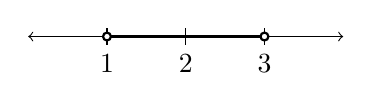
\begin{tikzpicture}
\draw[<->] (0,0) -- (4,0) ;
\foreach \x in  {1,2,3}
\draw[shift={(\x,0)},color=black] (0pt,3pt) -- (0pt,-3pt);
\foreach \x in {1,2,3}
\draw[shift={(\x,0)},color=black] (0pt,0pt) -- (0pt,-3pt) node[below] 
{$\x$};
\node[draw, circle, thick, fill=white, minimum size=1mm, inner sep=0] at (1,0) {};
\node[draw, circle, thick, fill=white, minimum size=1mm, inner sep=0] at (3,0) {};
\draw[very thick    ] (1.05,0) -- (2.95,0);
\end{tikzpicture}
\end{center}

In $\mathbb{R}^2$, an open ball is the inside of a circle (not including the boundary). For example, $B_2((0,3))$ is the inside of the circle of radius $2$ centered at $(0,3)$.

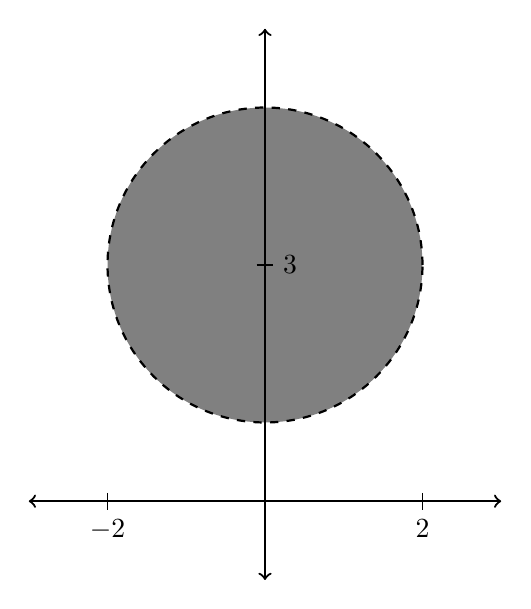
\begin{tikzpicture}
\draw[thick, dashed, fill=gray] (0,3) circle (2);
\draw[<->, thick] (-3,0) -- (3,0);
\draw[<->, thick] (0,-1) -- (0,6);

\foreach \x in {-2,2}
\draw[shift={(\x,0)},color=black] (0pt,3pt) -- (0pt,-3pt) node[below] 
{$\x$};

\draw[shift={(0,3)},color=black] (-3pt,0pt) -- (3pt,0pt) node[right] 
{$3$};
\end{tikzpicture}

In $\mathbb{R}^3$, and open ball is the inside of a sphere of radius (not including the boundary). For example, $B_1((0,0,0))$ is the inside of the sphere of radius $1$ centered at the origin.

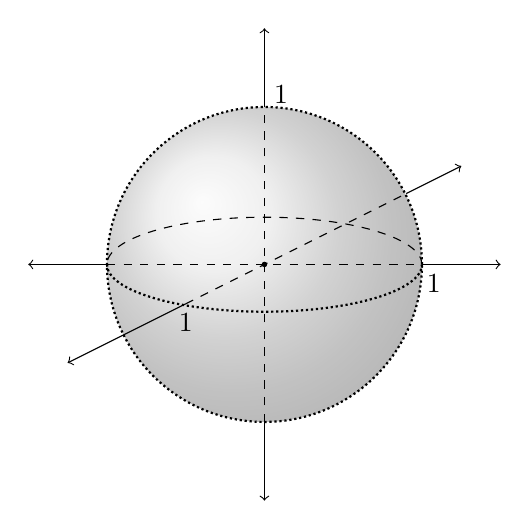
\begin{tikzpicture}
  \shade[ball color = gray!40, opacity = 0.4] (0,0) circle (2cm);
  \draw[thick, densely dotted] (0,0) circle (2cm);
  \draw[thick, densely dotted] (-2,0) arc (180:360:2 and 0.6);
  \draw[dashed] (2,0) arc (0:180:2 and 0.6);
  \fill[fill=black] (0,0) circle (1pt);
  
  \draw[<-] (-3, 0) -- (-2,0);
  \draw[dashed ] (-2,0 ) -- (2,0) node[below, xshift=1ex] 
{$1$};
  \draw[->] (2,0) -- (3,0);
  \draw[<-] (0, -3) -- (0,-2);
  \draw[dashed] (0,-2 ) -- (0,2) node[right, yshift = 1ex] 
{$1$};
  \draw[->] (0,2) -- (0,3);
  \draw[<-] (-2.5, -1.25) -- (-1,-0.5);
  \draw[dashed] (-1,-0.5) node[below] 
{$1$} -- (1.8, 0.9);
  \draw[->] (1.8, 0.9) -- (2.5, 1.25);
\end{tikzpicture}

Describe the following open balls:

In $\mathbb{R}^1$, $B_3(1)$ is the 
\begin{multipleChoice}
\choice[correct]{open interval}
\choice{inside of a circle}
\choice{inside of a sphere}
\end{multipleChoice}
 $(\answer[given]{-2},\answer[given]{4})$.
 
 In $\mathbb{R}^2$, $B_2((1,1))$ is the
 \begin{multipleChoice}
\choice{open interval}
\choice[correct]{inside of a circle}
\choice{inside of a sphere}
\end{multipleChoice}
of radius $\answer[given]{2}$ centered at $(\answer[given]{1}, \answer[given]{1})$.

In $\mathbb{R}^3$, $B_4((1,2,3))$ is the
\begin{multipleChoice}
\choice{open interval}
\choice{inside of a circle}
\choice[correct]{inside of a sphere}
\end{multipleChoice}
of radius $\answer[given]{4}$ centered at $(\answer[given]{1}, \answer[given]{2}, \answer[given]{3})$.
\end{foldable}
\end{example}

Now we can define open sets in general, using our new idea of open balls.

\begin{definition}
A set $U\subset \mathbb{R}^n$ is \emph{open} if for every $\mathbf{a}\in U$, there is a radius $r>0$ such that $B_r(\mathbf{a})\subset U$.
\end{definition}

In words, for any point $\mathbf{a}$ in $U$, we can find a radius $r$ small enough that the entire ball of radius $r$ centered at $\mathbf{a}$ is contained in $U$.

%PICTURE, OR VIDEO?

Even if we don't have an open set, it's possible that there might be some points in $U$ with this special property. We call these points interior point.

\begin{definition}
Let $U\subset \mathbb{R}^n$. A point $\mathbf{a}\in U$ is an \emph{interior point} if there is a radius $r>0$ such that $B_r(\mathbf{a})\subset U$.
\end{definition}

So, we can restate the definition of an open set as ``every point is an interior point.''

\begin{example}
\begin{foldable}
For each of the following, determine whether or not the set is open.

\begin{enumerate}
\item $\{(x,y)\,:\,x^2+y^2<1\}$ in $\mathbb{R}^2$
\begin{multipleChoice}
\choice[correct]{open}
\choice{not open}
\end{multipleChoice}			%VIDEO EXPLANATION
\item $\{(x,y)\,:\,x^2+y^2\leq 1\}$ in $\mathbb{R}^2$
\begin{multipleChoice}
\choice{open}
\choice[correct]{not open}
\end{multipleChoice}			%VIDEO EXPLANATION
\item $\mathbb{R}^2$ in $\mathbb{R}^2$
\begin{multipleChoice}
\choice[correct]{open}
\choice{not open}
\end{multipleChoice}			%VIDEO EXPLANATION
\item $\emptyset$ in $\mathbb{R}^n$
\begin{multipleChoice}
\choice[correct]{open}
\choice{not open}
\end{multipleChoice}			%VIDEO EXPLANATION
\item $\{(x,y)\,:\,x\geq 0\textrm{ and }y\geq 0\}$ in $\mathbb{R}^2$
\begin{multipleChoice}
\choice{open}
\choice[correct]{not open}
\end{multipleChoice}			%VIDEO EXPLANATION
\item $\{(x,y)\,:\,x<y\}$ in $\mathbb{R}^2$
\begin{multipleChoice}
\choice[correct]{open}
\choice{not open}
\end{multipleChoice}			%VIDEO EXPLANATION
\end{enumerate}
\end{foldable}
\end{example}

We finish this section by proving an important result about open sets: that the union of a collection of open sets is itself an open set.

\begin{theorem}
Suppose $\{U_i\}$ is a collection of open sets, where each $U_i$ is open. Let $U=\bigcup U_i$, the union of all the $U_i$. Then $U$ is an open set.
\end{theorem}

\begin{proof}
\begin{unfoldable}
Let $\mathbf{a}\in U$. We will show that $\mathbf{a}$ is an interior point.

Since $\mathbf{a}\in U=\bigcup U_i$, there is some $i$ such that $\mathbf{a}\in U_i$. Since $U_i$ is open, there is a radius $r>0$ such that $B_r(\mathbf{a})$ is contained entirely in $U_i$. Then, since $U_i \subset U$, we have that $B_r(\mathbf{a})\subset U$. This shows that $\mathbf{a}$ is an interior point, and that $U$ is an open set.

%VIDEO EXPLANATION
\end{unfoldable}
\end{proof}

\section{Closed Sets}

We now introduce closed sets, which are defined via their relationship to open sets.

\begin{definition}
A set $X\subset \mathbb{R}^n$ is \emph{closed} if its complement is open.
\end{definition}

Recall that the \emph{complement} of a subset $X$ of $\mathbb{R}^n$ consists of the elements of $\mathbb{R}^n$ which are not in $X$. That is,
\[
\mathbb{R}^n\setminus X = X^C = \{\mathbf{x}\in\mathbb{R}^n\,:\,\mathbf{x}\in X\}.
\]
$\mathbb{R}^n\setminus X$ and $X^C$ are both common notations for complements. $X^C$ has the advantage of being succinct, while $\mathbb{R}^n\setminus X$ has the advantage of referring to the larger set $\mathbb{R}^n$, which can help avoid confusion.

We now give a couple examples of closed sets.

\begin{example}
\begin{foldable}
The closed interval $[1,3]$ is a closed set in $\mathbb{R}$, since its complement, $(-\infty, 1)\cup (3,\infty)$, is an open set.

The set $\{(x,y)\,:\,x^2+y^2\leq 1\}\subset \mathbb{R}^2$, since its complement, $\{(x,y)\,:\,x^2+y^2> 1\}$, is an open set.
\end{foldable}
\end{example}

It's very important to remember that, even though closed sets are defined in relation to open sets, {\color{red}``closed'' is not the same as ``not open''}. It is possible for a set to be neither closed nor open, and it's possible for a set to be both open and closed.

\begin{example}
\begin{foldable}
The interval $[0,1)$ in $mathbb{R}$ is neither closed nor open. It is not open, since $0\in [0,1)$ is not an interior point. It is also not closed, because its complement, $(-\infty, 0)\cup [1,\infty)$, is not open ($1$ is not an interior point).

$\mathbb{R}^2$ (in $\mathbb{R}^2$) is both closed and open. We've seen that its open, and we've seen that its complement, $\emptyset$, is also open. Hence $\mathbb{R}^2$ is both open and closed.
\end{foldable}
\end{example} 

We've used the word ``boundary'' to refer to the ``edge'' of a set. This intuitive idea is useful in working with example, however we do need a rigorous definition of the boundary of a set, which we now give.

\begin{definition}
A point $\mathbf{x}\in\mathbb{R}^n$ is a \emph{boundary point} of a set $X\in \mathbb{R}^n$ if every $B_r(\mathbf{x})$ (for $r>0$) contains both points in $X$ and points not in $X$.

The set of all boundary points of $X$ is called the \emph{boundary} of $X$.
\end{definition}

\begin{example}
\begin{foldable}
The boundary of $\{(x,y)\,:\,x^2+y^2<1\}\subset\mathbb{R}^2$ is $\{(x,y)\,:\,x^2+y^2=1\}$. %VIDEO

The boundary of the interval $(0,1]\subset\mathbb{R}$ is $\{0,1\}$.
\end{foldable}
\end{example}

From working with examples of open and closed sets, you may have guessed that closed sets tend to contain their boundary points, while open sets do not. This is supported by the following theorem.

\begin{theorem}
A set $X\subset\mathbb{R}^n$ is closed if and only if it contains all of its boundary points.
\end{theorem}

\begin{proof}
\begin{unfoldable}
I'm not sure if I actually want to prove this...
\end{unfoldable}
\end{proof}

\begin{example}
\begin{foldable}
Practice identifying closed/open/neither/both.
\end{foldable}
\end{example}

\section{Connected Sets}

We now define what it means for a set to be path-connected. This is generally consistent with your intuitive idea of what ``connected'' should mean, but we are now able to make this mathematically rigorous.

\begin{definition}
A set $X\subset \mathbb{R}^n$ is path-connected if any two points can be connected by a path which lies entirely in $X$.
\end{definition}

\begin{example}
\begin{foldable}
For each of the following sets, determine whether or not they are path-connected.

IMAGE
\begin{multipleChoice}
\choice[correct]{path-connected}
\choice{not path-connected}
\end{multipleChoice}

IMAGE
\begin{multipleChoice}
\choice[correct]{path-connected}
\choice{not path-connected}
\end{multipleChoice}

IMAGE
\begin{multipleChoice}
\choice{path-connected}
\choice[correct]{not path-connected}
\end{multipleChoice}
\end{foldable}
\end{example}

\section{Simply Connected Sets}

The last topological concept we will cover is when a path-connected set is ``simply connected.'' Intuitively, this depends on whether or not the set has holes. Our definition for simply connected is a bit hand wavy, but this will serve our purpose just fine. It can be made rigorous using continuous maps. (INCLUDE THIS SOMEWHERE?)

\begin{definition}
A path-connected set $X\subset\mathbb{R}^n$ is \emph{simply connected} if any closed path (i.e., loop) can be shrunk to a point, where the shrinking occurs entirely in $X$.
\end{definition}

Note that a set needs to be path-connected in order to be considered simply connected.

\begin{example}
\begin{foldable}
For each of the following sets, determine whether or not they are simply connected.

$\mathbb{R}^2\setminus\{(0,0)\}$
IMAGE
\begin{multipleChoice}
\choice{simply connected}
\choice[correct]{not simply connected}
\end{multipleChoice}

$\mathbb{R}^2$
IMAGE
\begin{multipleChoice}
\choice[correct]{simply connected}
\choice{not simply connected}
\end{multipleChoice}

$\{(x,y,z)\,:\,x^2+y^2+z^2=1\}$
IMAGE
\begin{multipleChoice}
\choice[correct]{simply connected}
\choice{not simply connected}
\end{multipleChoice}

A torus (the surface of a donut)
IMAGE
\begin{multipleChoice}
\choice{simply connected}
\choice[correct]{not simply connected}
\end{multipleChoice}
\end{foldable}
\end{example}

\section{Conclusion}

In this activity, we introduced the following topological terms.
\begin{itemize}
\item open ball
\item open set
\item interior point
\item closed set
\item boundary point
\item boundary of a set
\item path-connected
\item simply connected
\end{itemize}

We also established the following results.
\begin{itemize}
\item The union of a collection of open sets is itself open.
\item A set is closed if and only if it contains all of its boundary points.
\end{itemize}

These terms will allow us to correctly state some theorems about vector fields, which have special requirements on the domain. These theorems will be covered in the next two activities.

\end{document}